\documentclass[11pt,a4paper]{article}
\usepackage{shared-style}
\usepackage{graphicx}
\usepackage{hyperref}

\shorttitle{Database Performance Analysis and Profiling}
\shortauthors{Adam Maltoni, Ibón de Mingo}

\begin{document}

\papertitle{Database Performance Analysis and Profiling}
\paperauthors{Adam Maltoni, Ibón de Mingo}
\paperdate{October 2024}

\begin{abstract}
In the current context of software development and data analysis, the efficient handling of large volumes of information is essential to guarantee optimal performance in applications and services. This project aims to compare and analyze the performance of various database management systems (DBMS), using CRUD (Create, Read, Update, Delete) operations to measure resource usage such as execution time and memory in massive data ingestion scenarios.
\end{abstract}

\tableofcontents
\newpage

\section{Introduction}
In the current context of software development and data analysis, the efficient handling of large volumes of information is essential to guarantee optimal performance in applications and services. This project aims to compare and analyze the performance of various database management systems (DBMS), using CRUD (Create, Read, Update, Delete) operations to measure resource usage such as execution time and memory in massive data ingestion scenarios.

For this analysis, we will work with four database systems: SQLite3, DuckDB, PostgreSQL, and MongoDB. Each of these systems presents different characteristics, advantages, and disadvantages that will be explored through the development of a set of tools that automate the generation of synthetic data and performance profiling. Additionally, the impact of caching and indexing mechanisms to optimize information access will be evaluated.

The ultimate goal is to provide a comparative analysis of the performance of the mentioned DBMSs, allowing us to draw conclusions that guide the choice of a suitable system for different data applications. Throughout this document, we will explain the methodology used, the results obtained, and the conclusions derived from the performance profiling.

\section{Data Generation and Loading}
We begin with the data generation, for which we used the Faker library to create two datasets. The first contains user information (name, unique ID, email, mobile phone, landline, address, etc.), and the second contains vehicle data (license plate, chassis number, manufacturer, year, model, and category). Both sets are related by the user's ID, who is the owner of the car. Subsequently, a third dataset called \textit{mix} is created, in which within each user's data, in JSON format, a list of their owned cars is included. This table will be used to facilitate queries in MongoDB.

The code is structured into three classes: \texttt{UserProvider}, \texttt{VehicleProvider}, and \texttt{MasterProvider}. Each class is responsible for generating a dataset. In this way, we manage to separate responsibilities, which facilitates the scalability and maintainability of the code.

The \texttt{UserProvider} class is responsible for generating data related to users, such as names, unique IDs, emails, phone numbers, and addresses. It is of utmost importance that IDs are unique since they will be the primary and foreign keys of the relational database tables. As we seek synthetic data that resembles reality as much as possible, we have also ensured that other fields like phone or email are unique. Regarding each user's address, care has been taken to match zip codes with the municipality and that the municipality is located in the generated province. To obtain the zip codes, the CSV dataset indicated in the project guidelines' references was used.

The \texttt{VehicleProvider} class is in charge of generating vehicle data, such as license plates, chassis numbers, and car characteristics. In generating license plates, the code adjusts the license plate format (old: before or during 2000; modern: after 2000) based on the vehicle's manufacturing year, replicating the real format of Spanish license plates. Just like for users, we tried to generate realistic data, so some attributes like the chassis number or VIN (primary key in vehicles) and the license plate are unique values in the dataset. For models, manufacturers (brands), and years, we relied on another sample CSV that we generated from about 300 observations of popular cars.

Finally, the \texttt{MasterProvider} class unifies user and vehicle generation, internally creating an instance of \texttt{UserProvider} and another of \texttt{VehicleProvider}. Through the \texttt{generate} method, the user and vehicle lists are formed together.

Once the data is generated, it is passed to CSV and JSON; this step is key as it will allow us to insert the data into the different DBMSs. But before that, we create the \texttt{merge\_data} function. With this function, we merge users and their assigned vehicles into a single list as a list of nested documents. This function is crucial for data handling in MongoDB as it facilitates queries where \texttt{JOINS} are needed.

To create the CSVs, vehicle and user data are used, and two independent CSVs are created with the information of each. To carry out this task, private functions are employed for each file. The CSV data will be inserted into relational databases.

On the other hand, JSON files are generated. We use an internal function \texttt{\_data\_to\_json}; with this design decision, we encapsulate JSON writing functionality. In JSON, we generate three different files: users, vehicles, and mix (data from the \texttt{merge\_data} function). These files will be inserted into MongoDB since it is a document-based database model.

\section{Table Creation and CRUD Operations on the Databases}
After generating the different files with the data, data ingestion is carried out in the various DBMSs. For relational databases, it is necessary to previously define the data schema; conversely, MongoDB, being a document database, is more flexible and accepts any data schema, so we will perform the ingestion directly.

To create the structure of relational databases, we designed a function called \texttt{create\_tables}. The first thing this function does is ensure that the tables to be created do not exist. To do this, via an internal function, the tables to be generated are deleted if they exist. For PostgreSQL, we use the \texttt{CASCADE} method to ensure the operation is carried out successfully. Finally, the table structure is created by defining the types of each attribute, indicating the primary keys (ID and chassis number), defining the attributes that must be unique, and referencing the ID of users owning cars in the vehicles table with the \texttt{user\_id} attribute. It is worth noting that it is important to delete vehicles before users to avoid violating referential integrity in the process.

With the structure defined in relational databases, we can start data ingestion. For this, we created a function called \texttt{insert\_data}. This function allows inserting data in three different ways: \texttt{chunk}, \texttt{at\_once}, and \texttt{one}. The \texttt{chunk} method inserts all data in batches of a predetermined size into the DBMS, which the user can also configure with a custom size. With \texttt{at\_once}, data is inserted directly into the DBMS, although in some cases like MongoDB (only 100k per insertion) they have a maximum insertion limit. Finally, the \texttt{one} method performs record-by-record insertion, opening and closing the connection for each insertion. The function also allows the creation of indexes in each DBMS; there is a parameter in the function called \texttt{use\_index: bool} that triggers index creation. In all cases, it is necessary to separate relational databases from MongoDB since the connection to the database is different.

As we will perform multiple data insertion operations throughout the tests and the project, we require a function to delete records from the databases. In this function, records are simply deleted from each DBMS using \texttt{DELETE}. We differentiate between MongoDB and the other DBMSs for logic implementation.

Next, we designed functions to perform read operations and updates in the various DBMSs. It should be mentioned that in all these functions, MongoDB\'s logic is separated from the other databases. Both the connection and the way to execute queries in MongoDB are very different from the other DBMSs, hence a different logic needs to be implemented. In the read functions (\texttt{SELECTS}), we created two functions, one that executes any read query and another that selects all records from the database. The update function is capable of executing any update query (\texttt{UPDATE}). We will use these functions later to design tests that allow us to compare different operations across each DBMS.

\section{Caches and Indexes}
Although databases are the central components of DBMSs for storage, they are not the only ones. Other noteworthy components include search indexes, a data structure that can improve operation speed by storing a unique pointer to each table row (like a PK), and caches, a high-speed data storage component or area (like RAM) used to temporarily store frequently accessed information.

However, both present or can present disadvantages. Indexes can slow down write operations (such as insertions, updates, and deletions), because every time data in an indexed column is modified, the index must also be updated to reflect the change, adding an extra load to the writing process. On the other hand, a cache can become obsolete if data within the database changes frequently, in addition to RAM being fast but expensive.

For this project, we tested both by creating indexes through \texttt{CREATE INDEX} statements (relational) or \texttt{collection.createIndex} (MongoDB, from Python), and using two different caches: Memcached (ref. in Bibliography) and a simple cache that works behind the scenes with a dictionary to compare and perform tests with both, implemented with the same interface as Memcached.

\section{Testing: Results and Conclusions}

\textbf{Note:} For this section, we used various memory and time profiling functions provided in the project guidelines. Some of these have undergone slight adaptations for the correct functioning of the entire program, which are detailed in Design Decisions.

\subsection{Testing Data Generation}
We start by performing tests for data generation. In them, we will measure the time it takes to execute the different data generation functions and the space they occupy in memory. For this, we will use the aforementioned profiling functions. We will measure the functions for generating users, generating vehicles, and for relating both tables.

\begin{figure}[h]
\centering
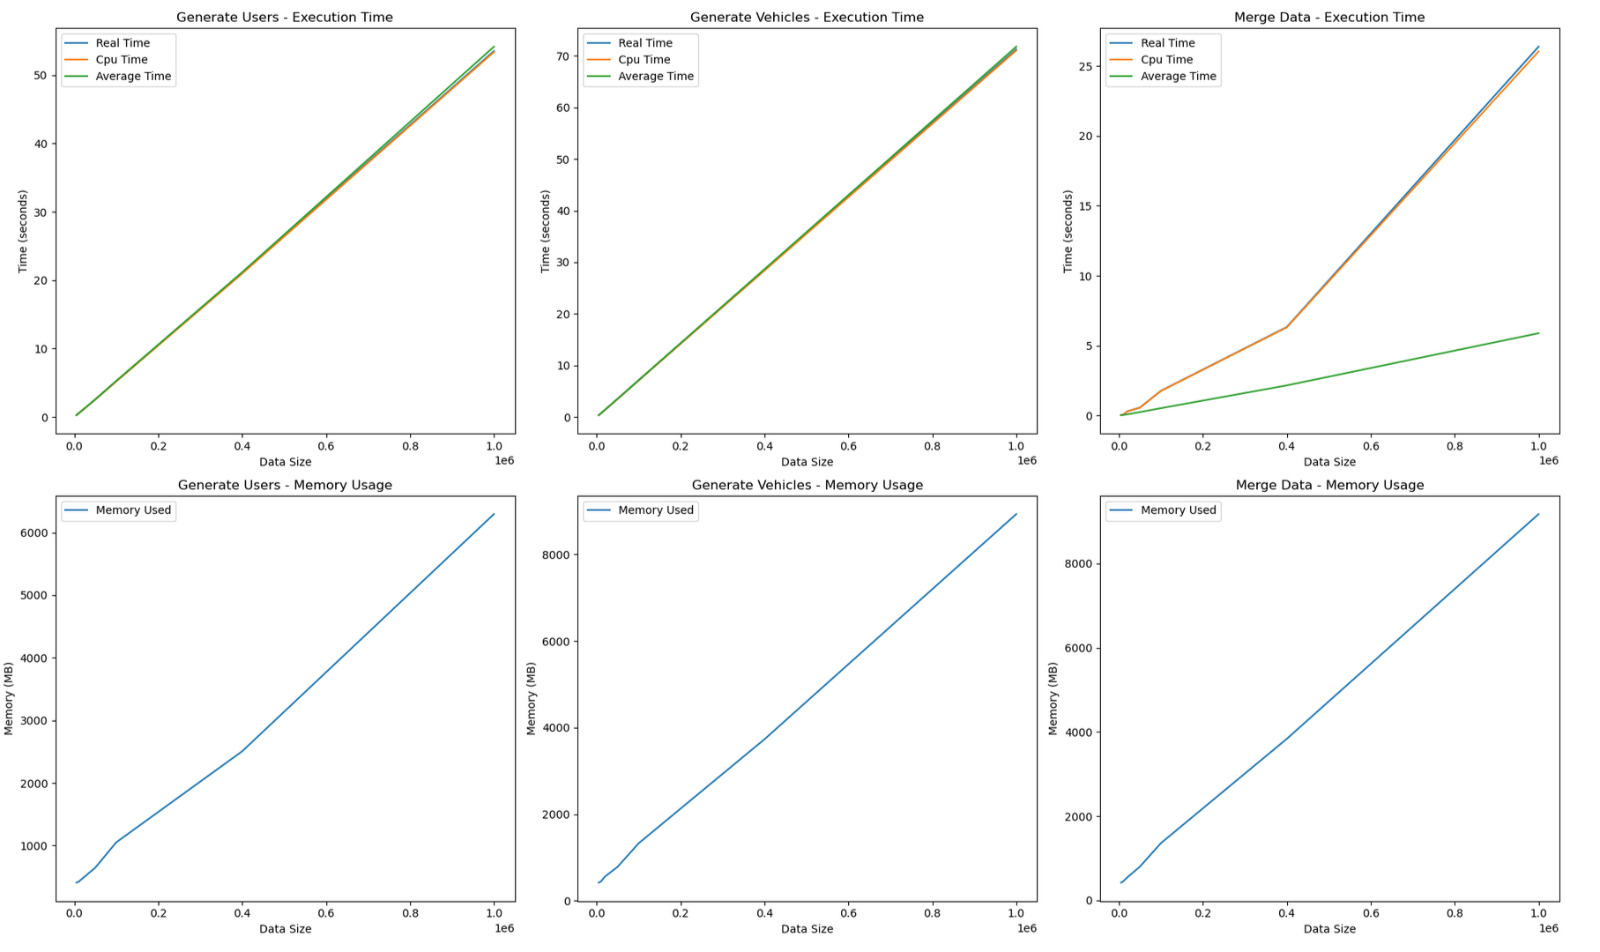
\includegraphics[width=0.8\textwidth]{img/page6_img1.png}
\caption{Plot of data generation testing}
\end{figure}

In the graphs, we observe that for both times and memory in all functions, the growth is linear as data size increases. In the \texttt{merge\_data} graph, we can observe that the average time is lower than the actual time; possibly due to external factors that caused an initial measurement spike.

We believe this is logical since in our code we make use of a sequential loop, that is, each record (user or vehicle) is generated within a for loop, iterating a number of times equal to the data size (number of entries). Therefore, if we double the size, the code will do twice the iterations. It should be mentioned that each operation to generate an ID, name, address, phone, or any field has a constant cost; therefore, if more records are generated, the total time increases proportionally.

\subsection{Testing CRUD Operations on Different DBMSs}
Next, we will run tests to measure both CPU and real times across the different DBMSs. We will start by making a joint comparison of all CRUD methods simultaneously, regardless of the DBMS, so that we can observe which type of operation consumes more time generally.

\begin{figure}[h]
\centering
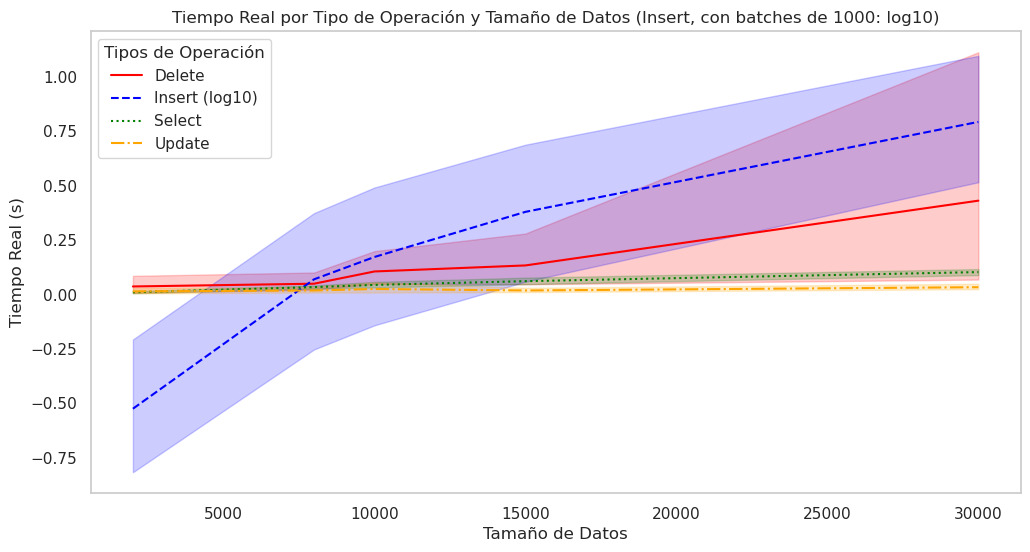
\includegraphics[width=0.8\textwidth]{img/page7_img1.png}
\caption{Comparative lineplot of temporal costs of various CRUD operations}
\end{figure}

To produce this graph, it was necessary to apply log10 to the times measured in insert since, clearly, it is the operation that takes the most time. Insertion time is linear since in the graph, with the logarithm applied, a logarithmic representation is seen. We consider it realistic because each individual insertion operation takes the same time as the others and the fact that there are many or few data entries in the database does not affect performance. The next operation that consumes the most time is deleting records from the database.

We believe this happens because DELETEs are performed in two databases and need to check primary keys to maintain referential integrity. It is for this very reason that the vehicle table is deleted before the users table, as previously mentioned.

In the next figure, besides comparing different operations, we decided to focus on insertion since it was the slowest in the first case. Therefore, in the tests, we decided to differentiate by insertion method to see its behavior in more detail.

\begin{figure}[h]
\centering
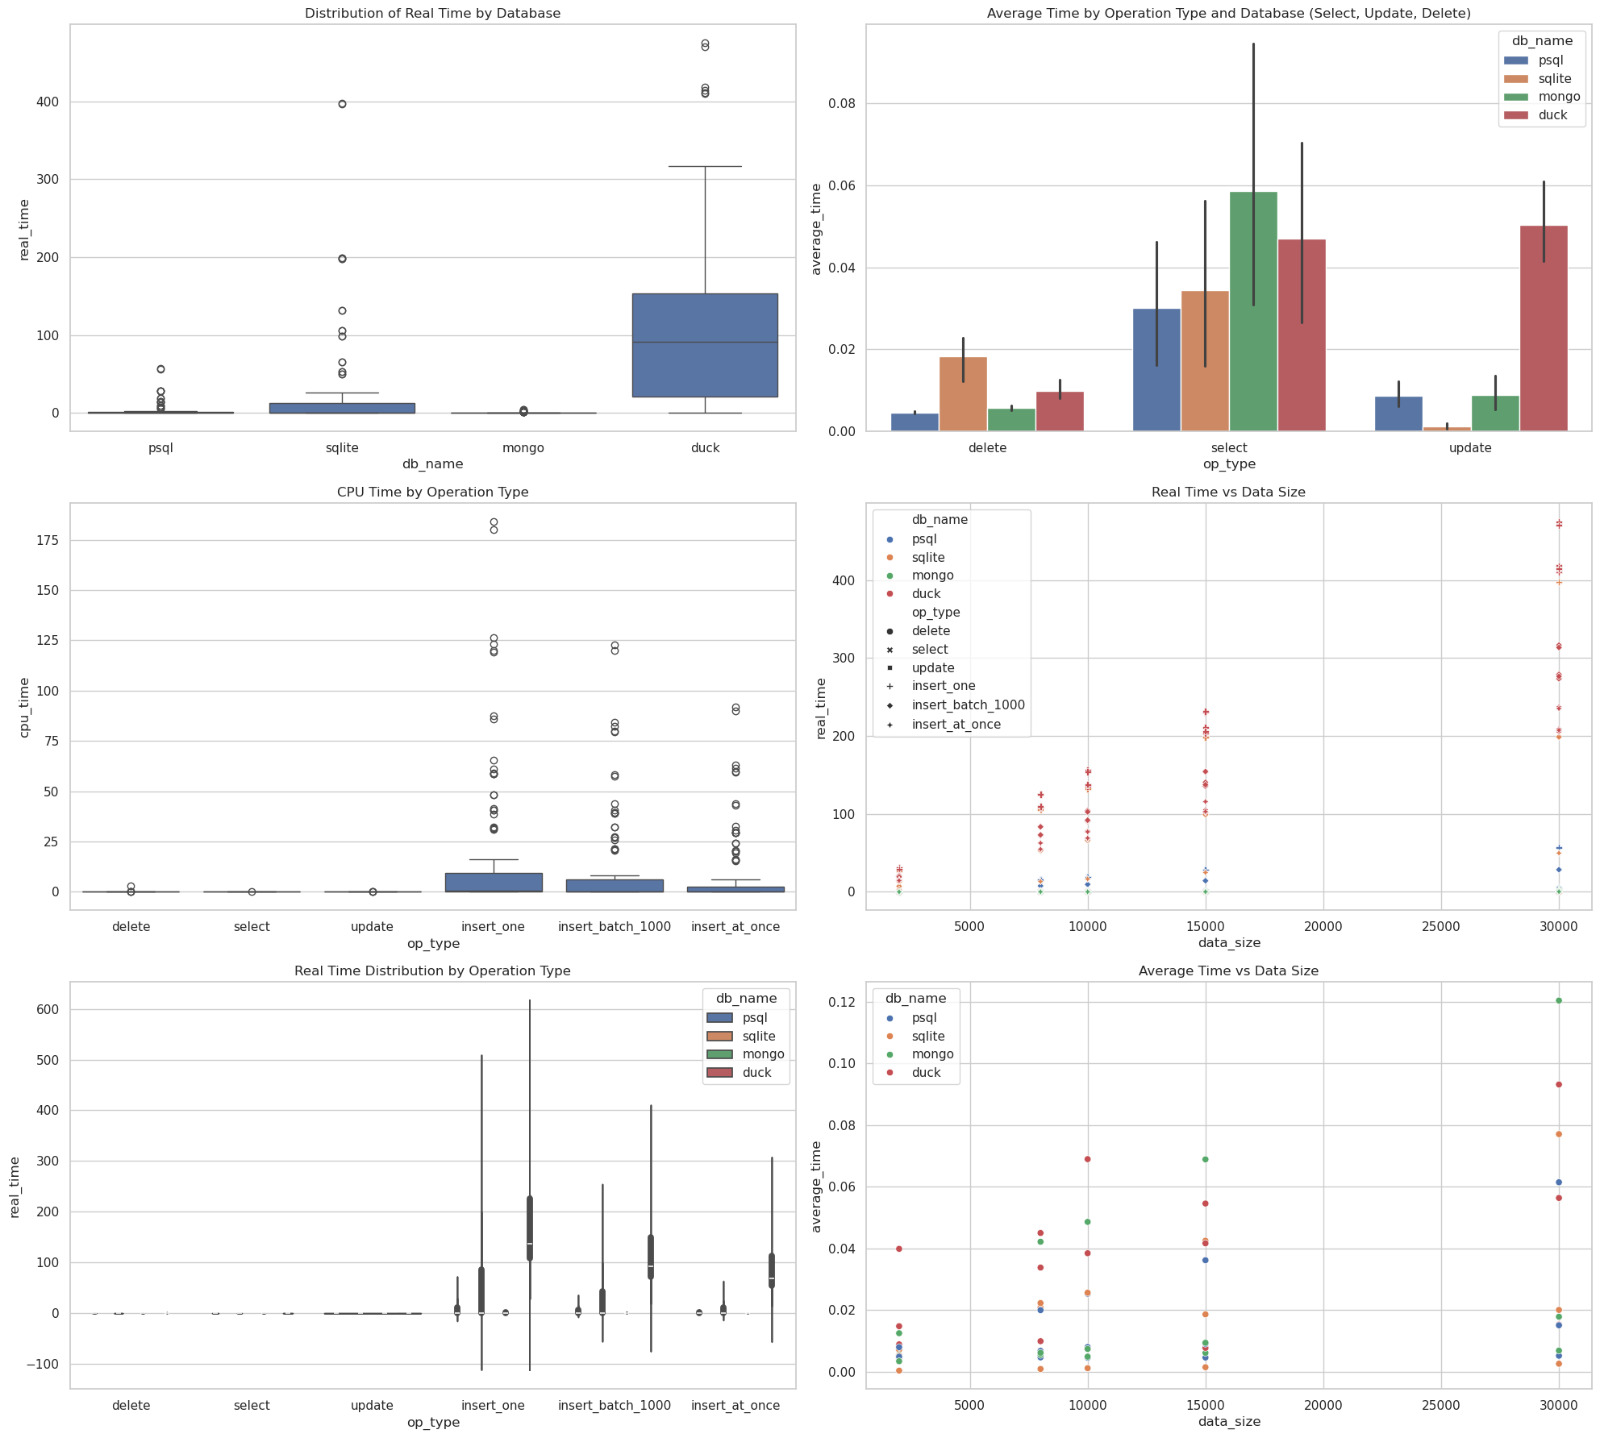
\includegraphics[width=0.8\textwidth]{img/page8_img1.png}
\caption{Various comparative subplots of various CRUD operations and different DBMSs}
\end{figure}

\textbf{Note:} It is worth noting that, in this other figure, the top-left plot obtains higher times for SELECTS. This is because we executed it with a slightly more complex query for this graph than before (\texttt{SELECT *}).

In the different graphs, it is clearly seen that the slowest insertion method is the \texttt{one} method since it opens and closes a connection every time it inserts data. On the contrary, the fastest method is \texttt{at\_once} since it inserts data directly. Leaving inserts aside, we observed that the slowest read operations are in MongoDB. We believe this happens because we ran the tests with referenced relationships, which is slower than having used embedded documents (\texttt{mix} table containing user and vehicle information together) and is slower than INNER JOINs in relational databases.

\begin{figure}[h]
\centering
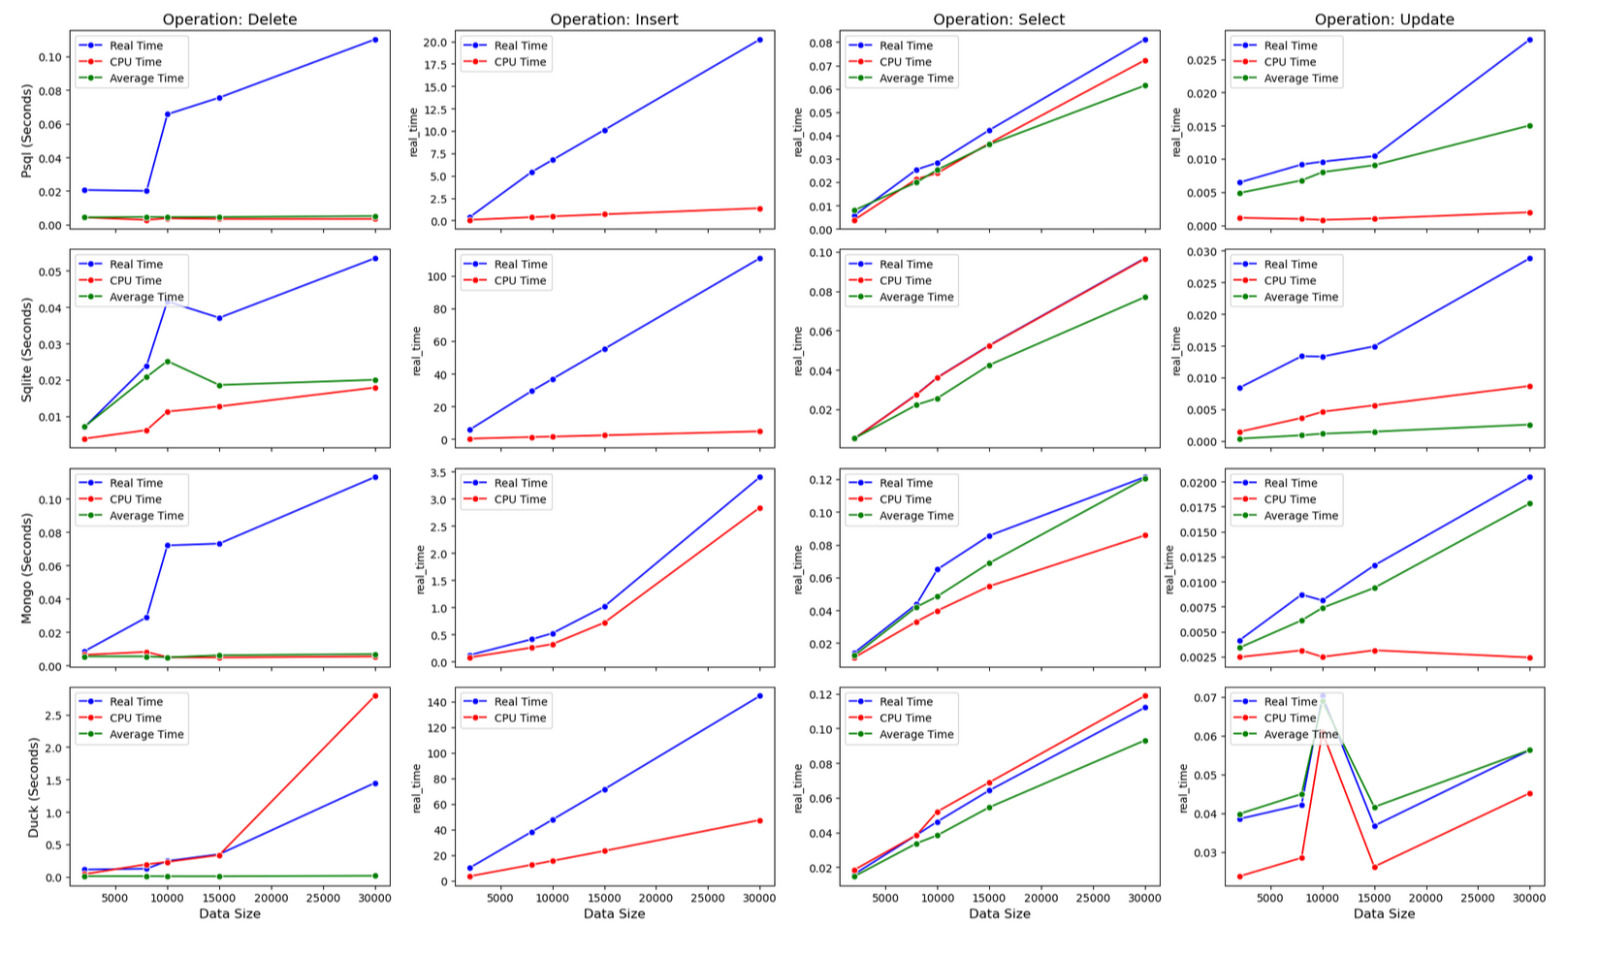
\includegraphics[width=0.8\textwidth]{img/page9_img1.png}
\caption{Another subplot comparing various CRUD operations and different DBMSs}
\end{figure}

\subsection{Testing Selection Queries and Cache Effectiveness}
In this section, we will focus on read operations, analyzing times with and without cache, seeing the influence of indexes in these operations, and analyzing the difference between the two methods to carry out read operations: \texttt{one} and \texttt{at\_once}. In both cases, all database records are read; the difference is that in the \texttt{one} method, the connection is opened and closed for each record while in \texttt{at\_once}, the connection remains active until the end of the process. These tests have been executed with different data sizes and multiple times, always observing the results and taking them into account for drafting this report.

For initial testing, we designed our own cache, which we decided to keep to compare with Memcached. In theory, we learned that Memcached uses a client-server architecture, and during the project, we had to connect to a server. It is possible that the server connection slowed down the cache process, which is why in some cases we achieved better performance with our own cache since it works locally.

\subsubsection{Queries on Primary Keys}
We perform two types of read operations: Joins and primary key searches. Join operations involve performing an INNER JOIN in relational databases (PostgreSQL, SQLite, and DuckDB), while in MongoDB, we will analyze the difference between using embedded relationships (using embedded documents) and referenced relationships (connecting different collections through references). In primary key searches, we will look for the primary key (ID) of the users table in each case.

We observed that clearly the \texttt{at\_once} method is much faster than the \texttt{one} method because constantly opening and closing the connection makes it much slower.

\begin{figure}[h]
\centering
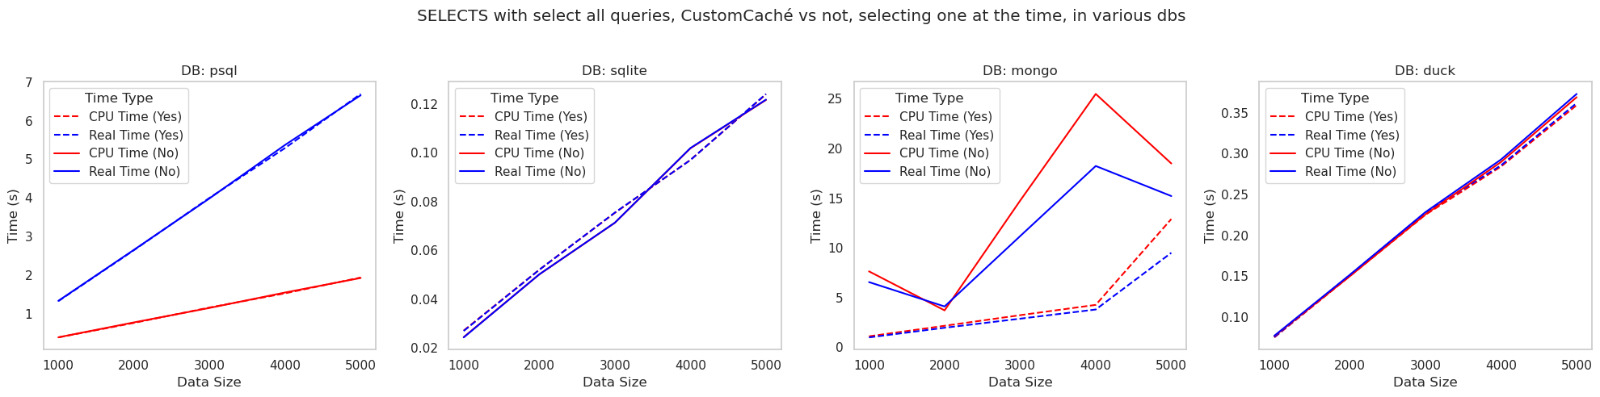
\includegraphics[width=0.8\textwidth]{img/page9_img2.png}
\caption{Subplots by DB, CustomCache vs without, one, on SELECT ALL queries}
\end{figure}

\begin{figure}[h]
\centering
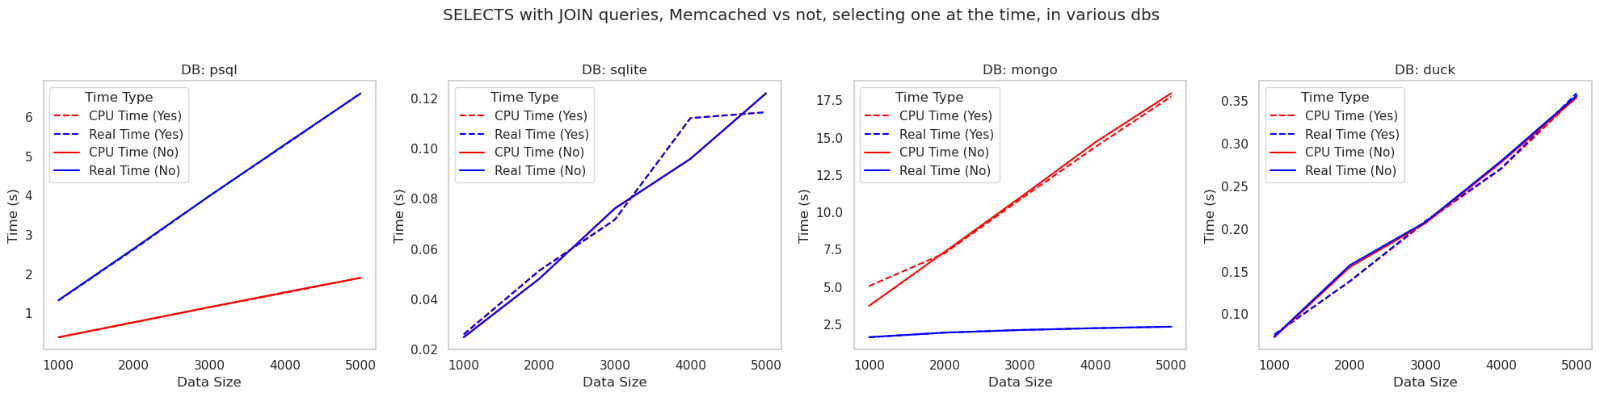
\includegraphics[width=0.8\textwidth]{img/page10_img1.png}
\caption{Subplots by DB, Memcached vs without, one, on SELECT ALL queries}
\end{figure}

\begin{figure}[h]
\centering
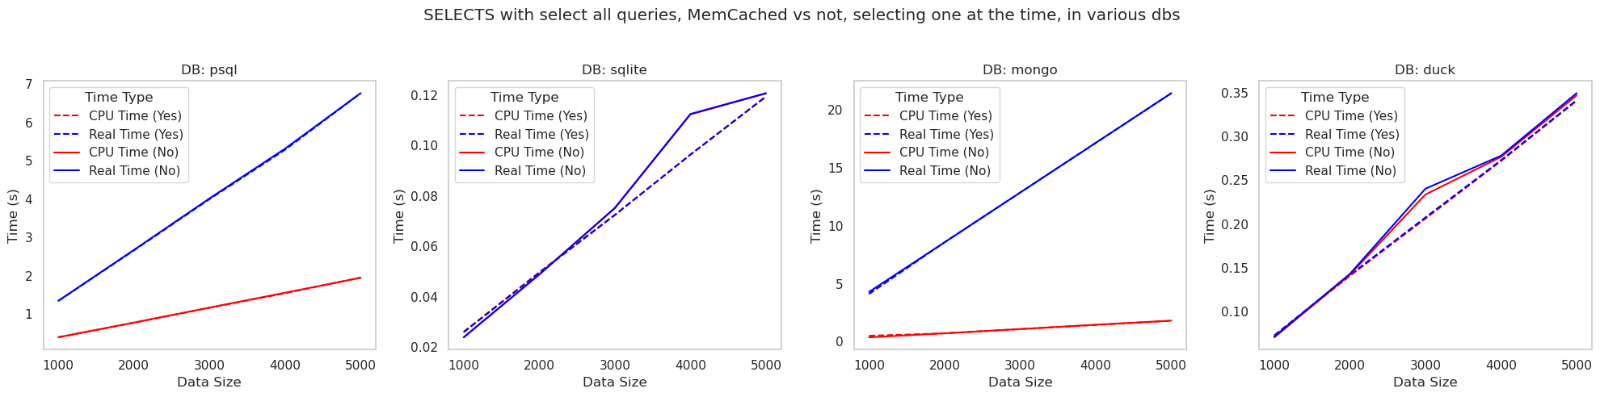
\includegraphics[width=0.8\textwidth]{img/page10_img2.png}
\caption{Subplots by DB, CustomCache vs without, at\_once, on SELECT ALL queries}
\end{figure}

\begin{figure}[h]
\centering
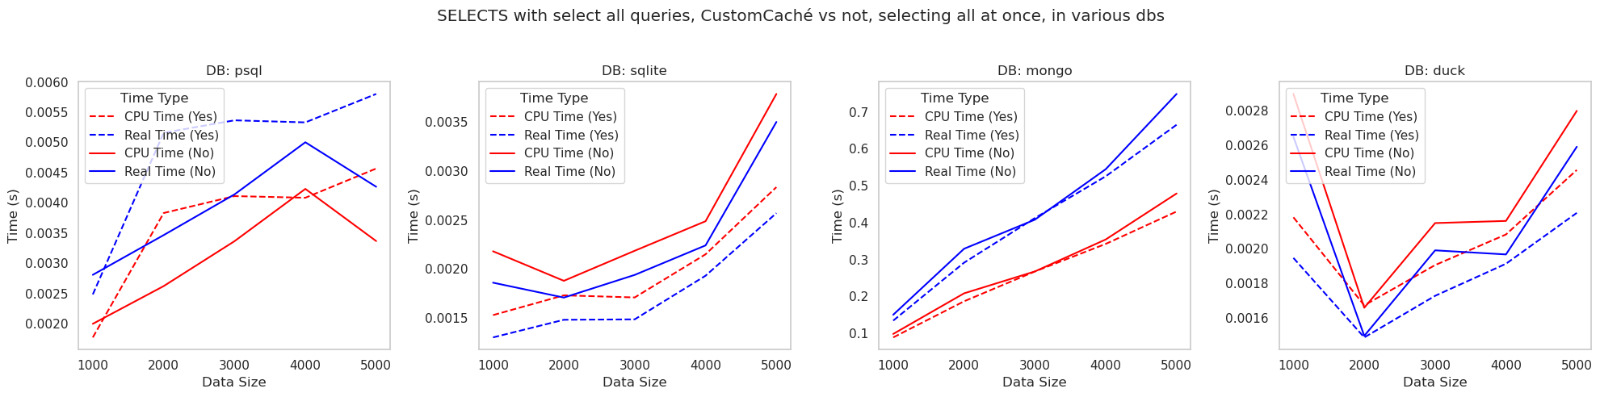
\includegraphics[width=0.8\textwidth]{img/page10_img3.png}
\caption{Subplots by DB, Memcached vs without, at\_once, on SELECT ALL queries}
\end{figure}

\subsubsection{Queries with JOIN}
\begin{figure}[h]
\centering
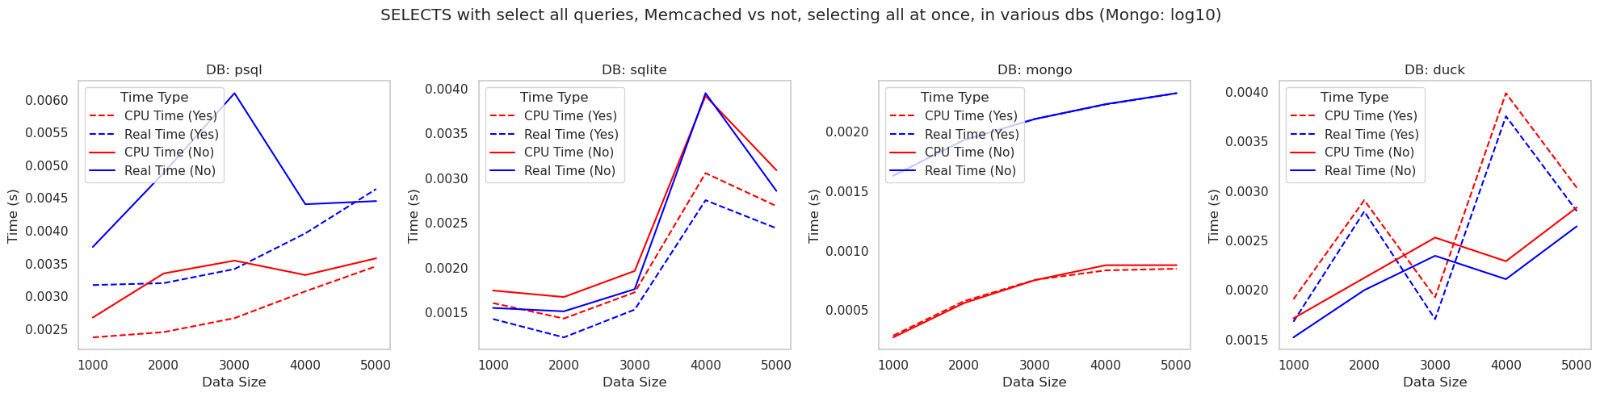
\includegraphics[width=0.8\textwidth]{img/page10_img4.png}
\caption{Subplots by DB, CustomCache vs without, one, on JOIN queries}
\end{figure}

\begin{figure}[h]
\centering
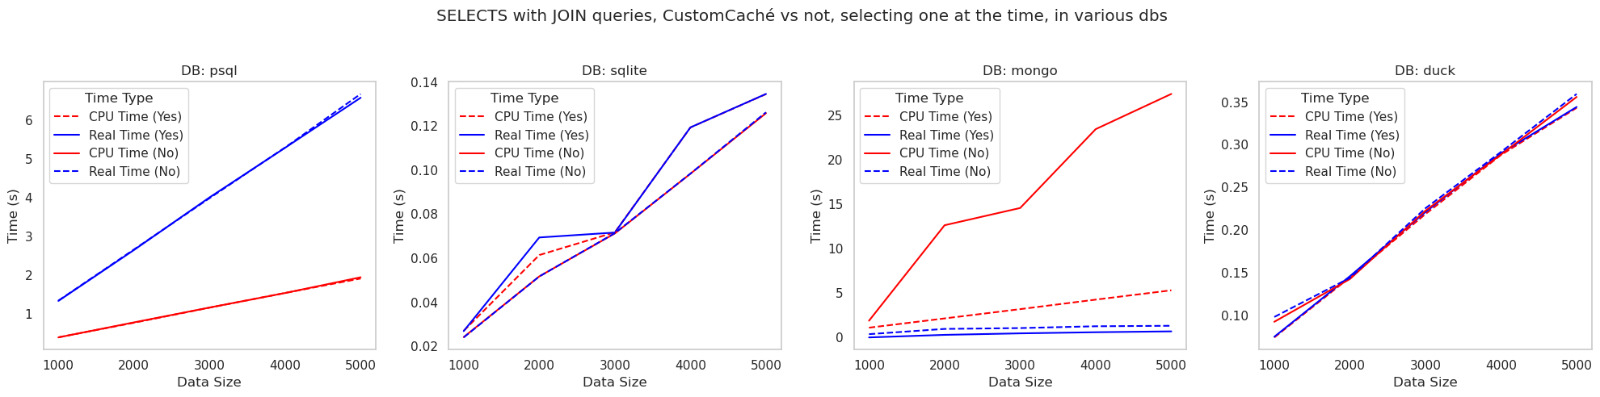
\includegraphics[width=0.8\textwidth]{img/page10_img5.png}
\caption{Subplots by DB, Memcached vs without, one, on JOIN queries}
\end{figure}

\begin{figure}[h]
\centering
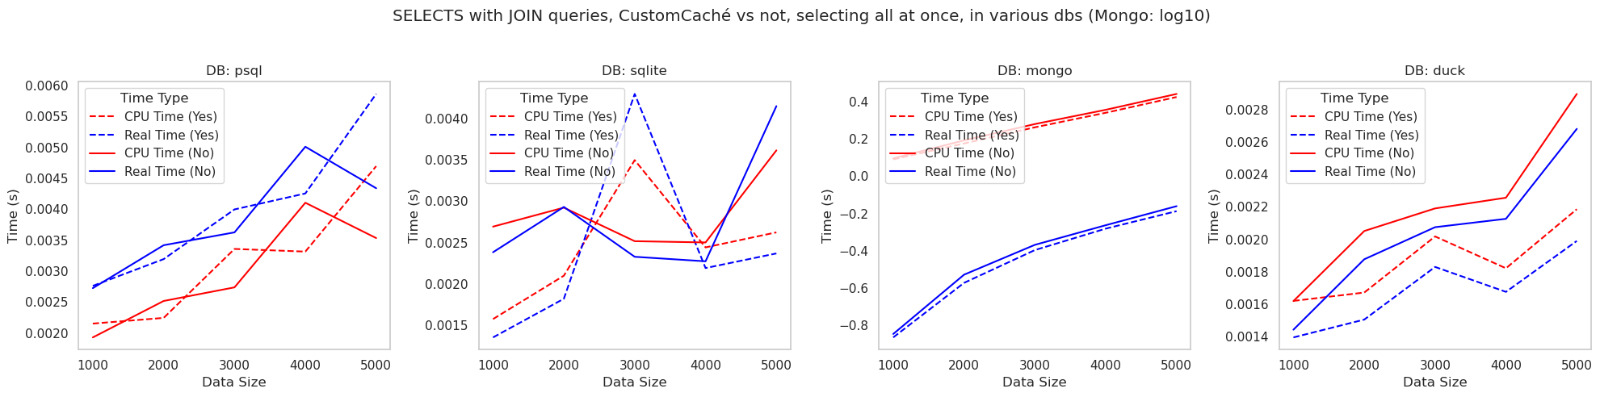
\includegraphics[width=0.8\textwidth]{img/page11_img1.png}
\caption{Subplots by DB, CustomCache vs without, at\_once, on JOIN queries}
\end{figure}

\begin{figure}[h]
\centering
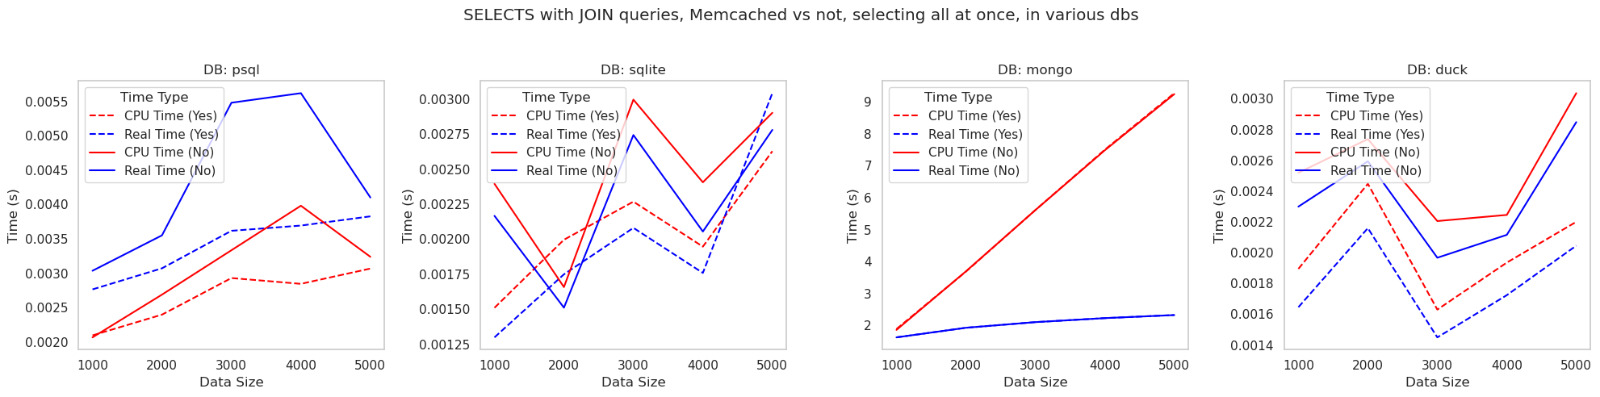
\includegraphics[width=0.8\textwidth]{img/page11_img2.png}
\caption{Subplots by DB, Memcached vs without, at\_once, on JOIN queries}
\end{figure}

As we previously explained, we perform tests with a join query that looks for the cars associated with each person found in the users table. In relational databases, we observed that this operation is quite well optimized, and in MongoDB, we noted that it is not designed to be fast in read operations with referenced relationships.

In PostgreSQL, INNER JOINs generally work fast. Investigating, we discovered that it uses an advanced query optimizer that chooses the best execution plan for performing joins. This matches our observations as we verified that PostgreSQL JOINs are quite fast compared to other DBMSs like MongoDB. With indexes on the JOIN, performance is significantly improved, reducing search time.

In SQLite, for queries with small data sizes (as in the graph), read operations are fast; however, as data size increased, it progressively lost efficiency.
In DuckDB, generally, read times in JOINs are low because, as mentioned in theory, DuckDB is designed to handle large data volumes and process joins efficiently. That is why we believe it is the fastest DBMS when reading. On the other hand, using indexes in DuckDB does not improve query performance since DuckDB uses other optimization methods.

After taking measurements in MongoDB, we concluded that MongoDB is not recommended for performing referenced relationships. Its performance with \ is much slower than INNER JOINs of SQL databases. We get much better performance when searching using embedded relationships since \ is unnecessary and all information is contained in the same document. However, we noticed that indexes in \ improved search performance, making it significantly faster.

All these operations were performed using cache and without cache. We verified that using the cache in most cases was beneficial since having the search stored meant there was no need to perform the query with the JOIN, which otherwise increases times.

\subsubsection{Queries on Primary Keys (Part 1)}
\begin{figure}[h]
\centering
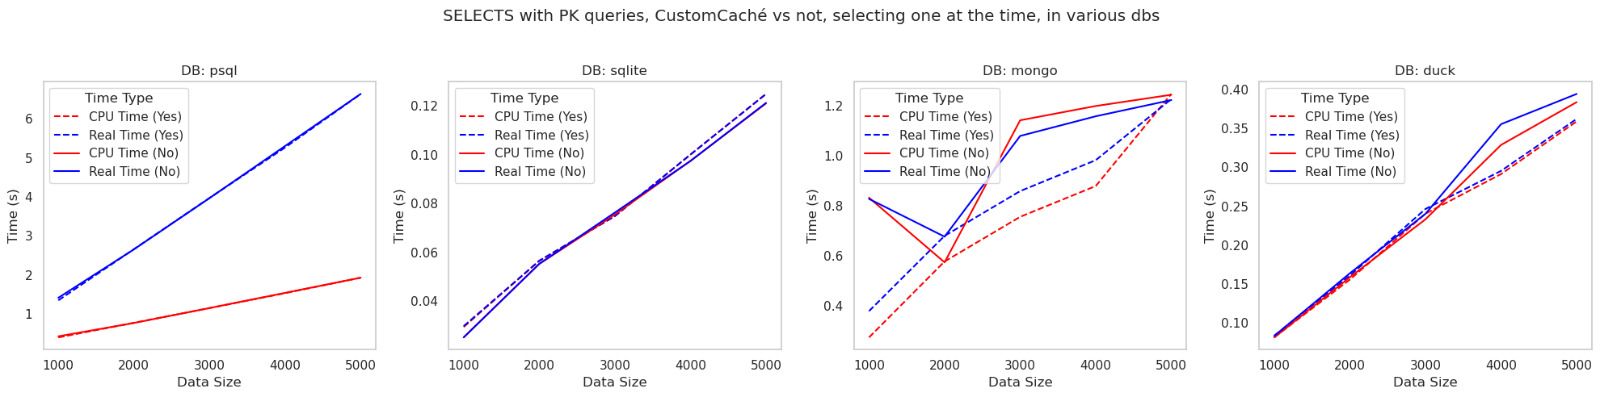
\includegraphics[width=0.8\textwidth]{img/page12_img1.png}
\caption{Subplots by DB, CustomCache vs without, one, on PK queries}
\end{figure}

\begin{figure}[h]
\centering
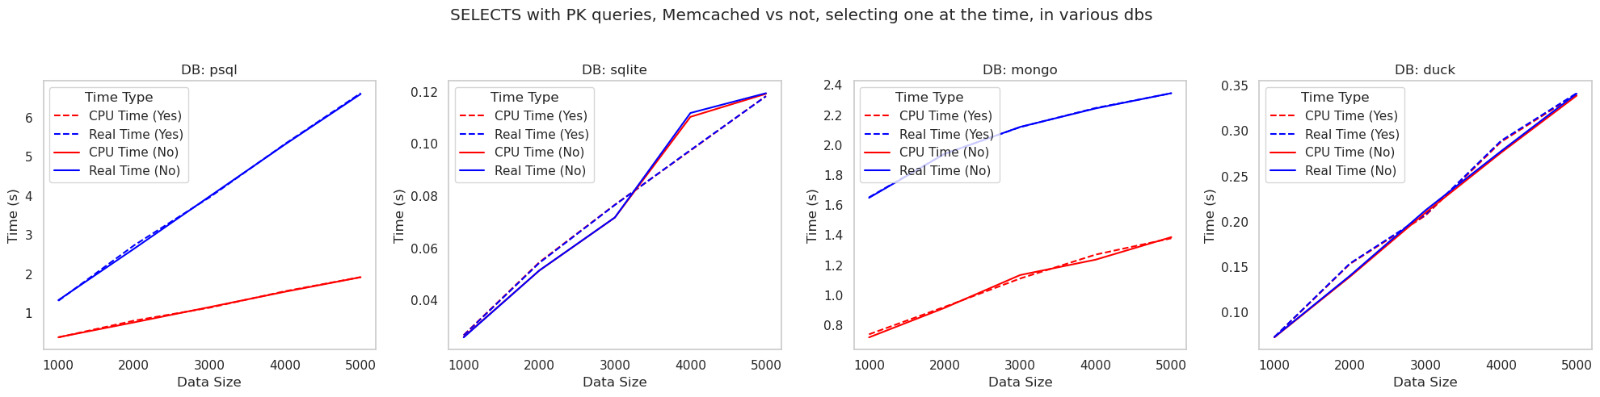
\includegraphics[width=0.8\textwidth]{img/page12_img2.png}
\caption{Subplots by DB, Memcached vs without, one, on PK queries}
\end{figure}

\begin{figure}[h]
\centering
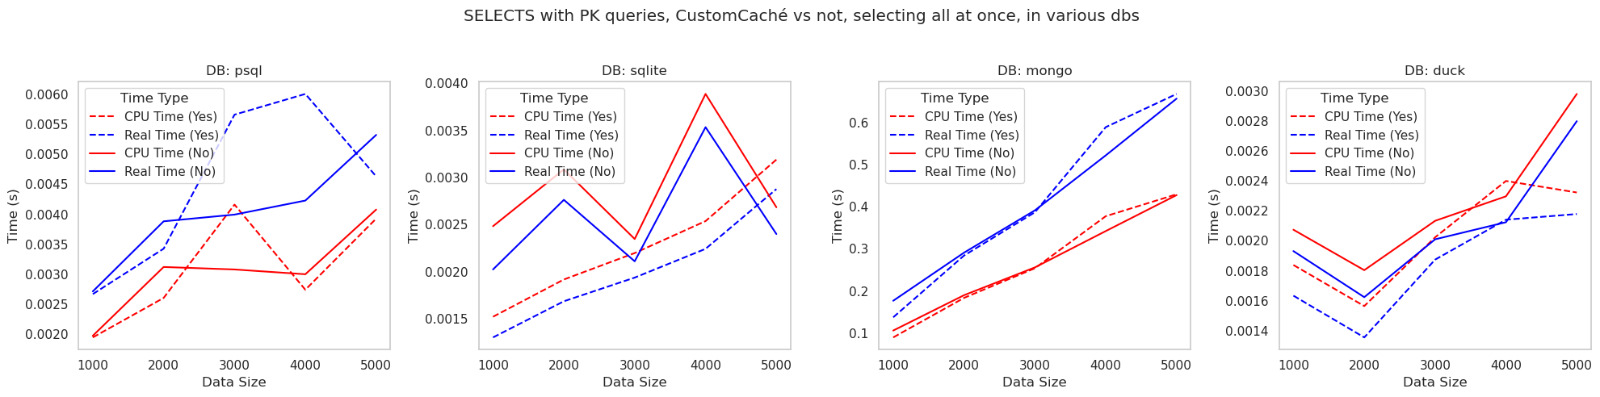
\includegraphics[width=0.8\textwidth]{img/page12_img3.png}
\caption{Subplots by DB, CustomCache vs without, at\_once, on PK queries}
\end{figure}

\begin{figure}[h]
\centering
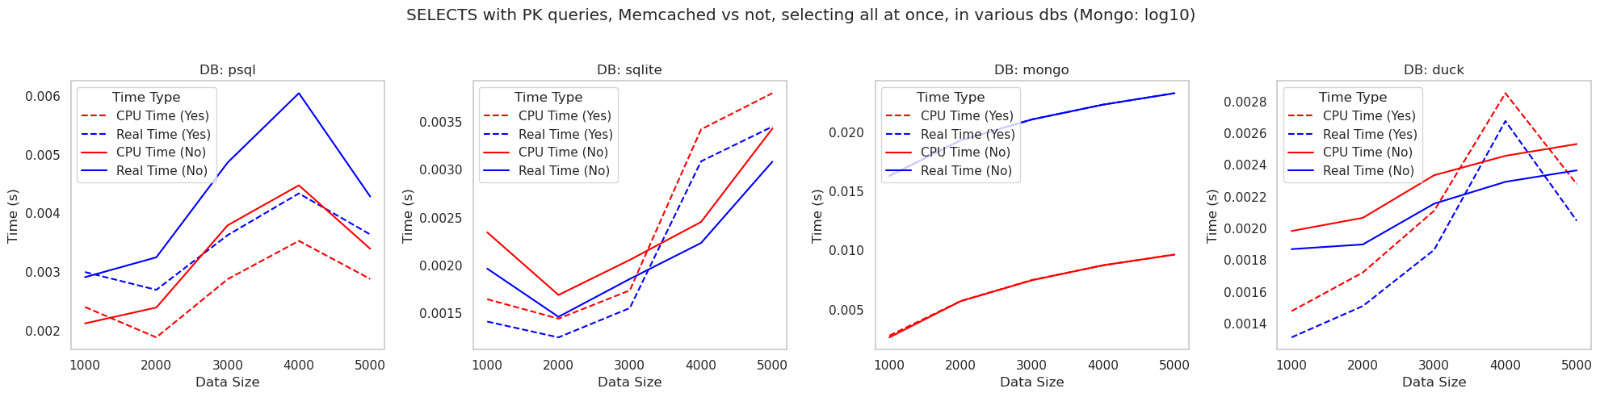
\includegraphics[width=0.8\textwidth]{img/page12_img4.png}
\caption{Subplots by DB, Memcached vs without, at\_once, on PK queries}
\end{figure}

In SQLite and PostgreSQL, primary key search turned out quite fast as they have mechanisms to optimize primary key searches that automatically create indexes on the primary key. Hence, manually creating indexes does not improve efficiency.

MongoDB does not really have a primary key, but it has an automatic unique key called \texttt{\_id}, which acts as a primary key. MongoDB automatically creates an index on this field, making searches on it extremely fast. On the other hand, since this column is already indexed, it makes no sense to create an index on the primary key.

DuckDB does not have a primary key system, so performing this query yields the same results as selecting each document. In this case, the use of indexes does improve performance since they are not automatically created with the primary key (it doesn\'t exist).

\subsubsection{Queries on Primary Keys (Part 2)}
\begin{figure}[h]
\centering
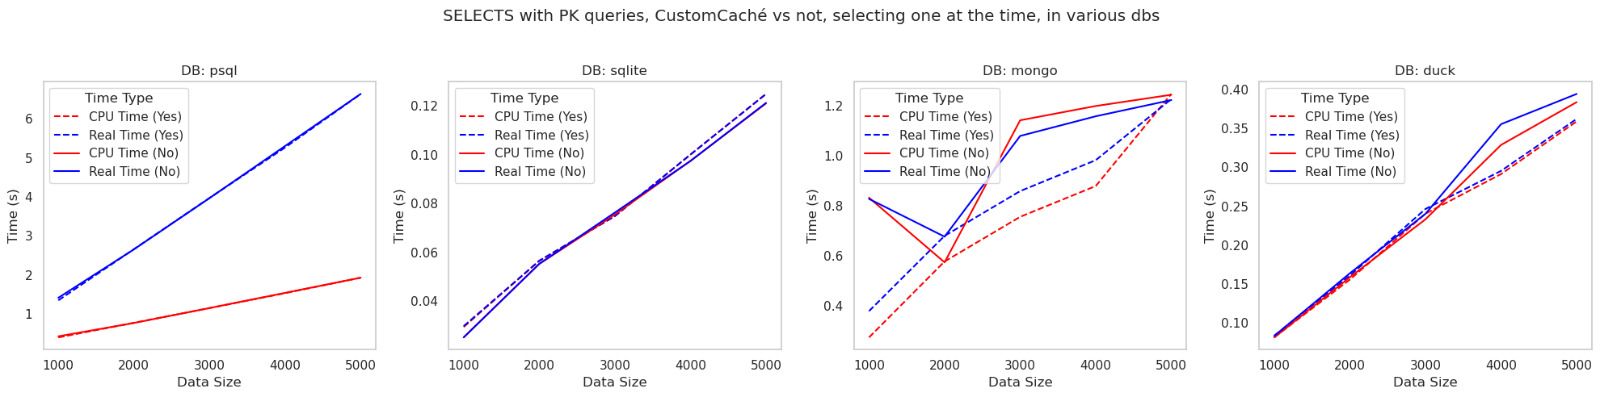
\includegraphics[width=0.8\textwidth]{img/page13_img1.png}
\caption{Subplots by DB, CustomCache vs without, one, on PK queries}
\end{figure}

\begin{figure}[h]
\centering
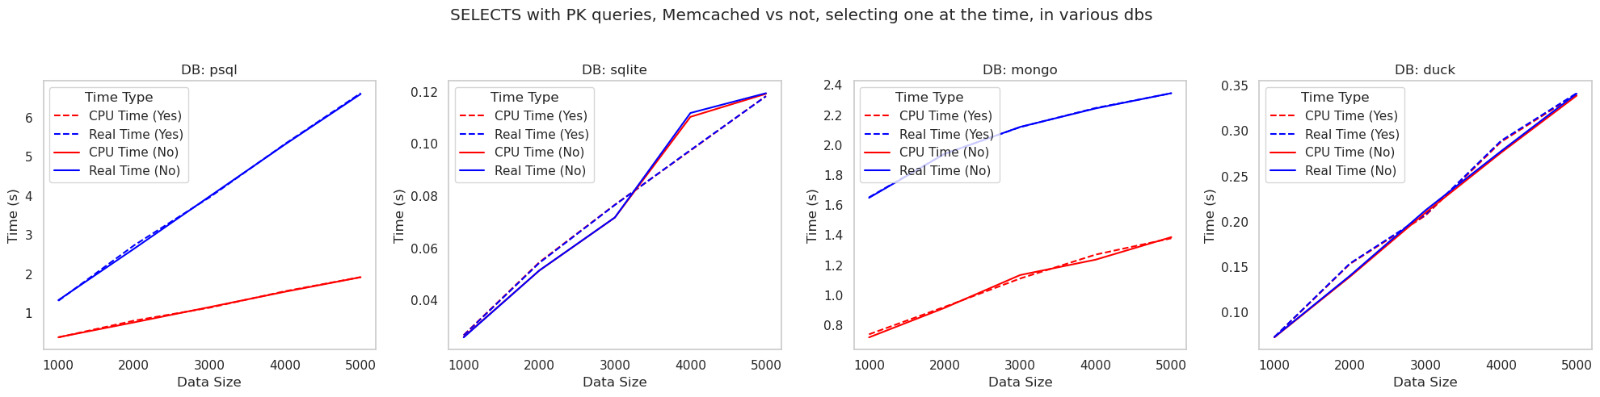
\includegraphics[width=0.8\textwidth]{img/page13_img2.png}
\caption{Subplots by DB, Memcached vs without, one, on PK queries}
\end{figure}

\begin{figure}[h]
\centering
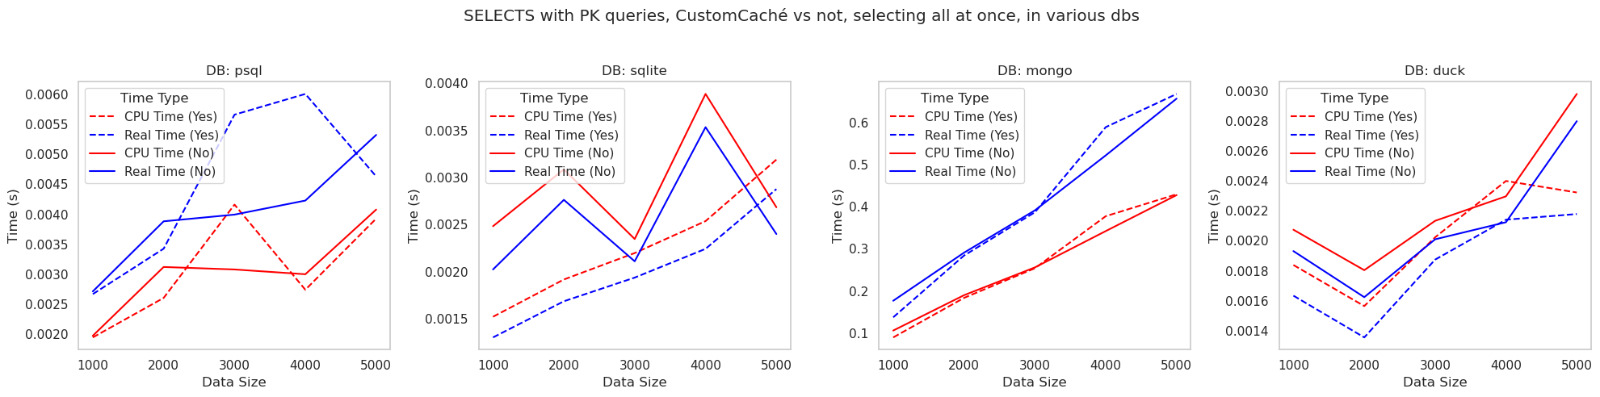
\includegraphics[width=0.8\textwidth]{img/page13_img3.png}
\caption{Subplots by DB, CustomCache vs without, at\_once, on PK queries}
\end{figure}

\begin{figure}[h]
\centering
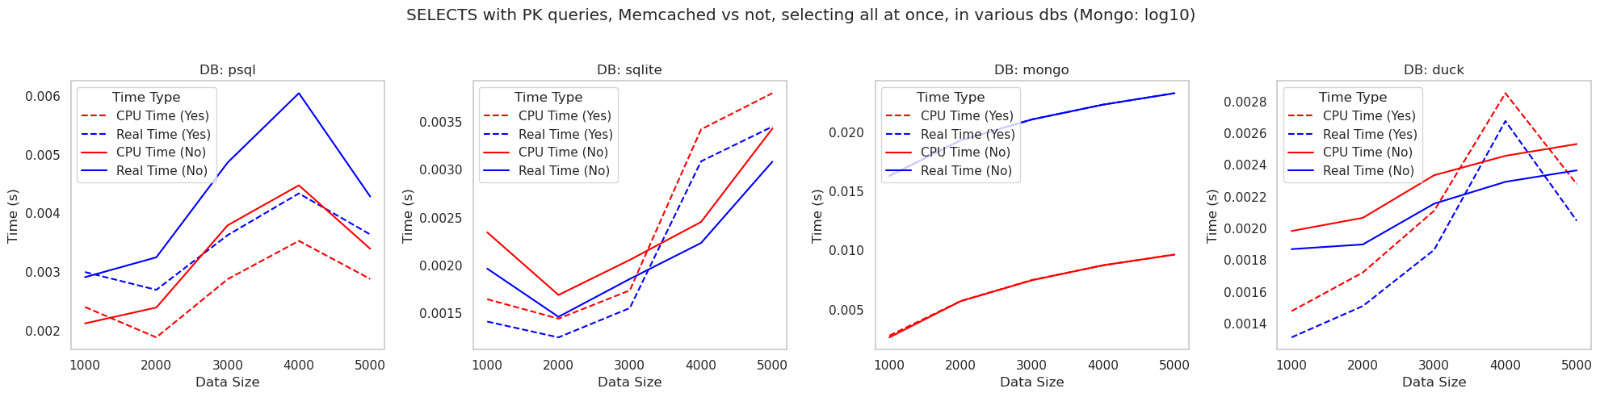
\includegraphics[width=0.8\textwidth]{img/page13_img4.png}
\caption{Subplots by DB, Memcached vs without, at\_once, on PK queries}
\end{figure}

In SQLite and PostgreSQL, primary key search turned out quite fast as they have mechanisms to optimize primary key searches that automatically create indexes on the primary key. Hence, manually creating indexes does not improve efficiency.

MongoDB does not really have a primary key, but it has an automatic unique key called \texttt{\_id}, which acts as a primary key. MongoDB automatically creates an index on this field, making searches on it extremely fast. On the other hand, since this column is already indexed, it makes no sense to create an index on the primary key.

DuckDB does not have a primary key system, so performing this query yields the same results as selecting each document. In this case, the use of indexes does improve performance since they are not automatically created with the primary key (it doesn\'t exist).

\subsection{Testing Update Queries}

\begin{figure}[h]
\centering
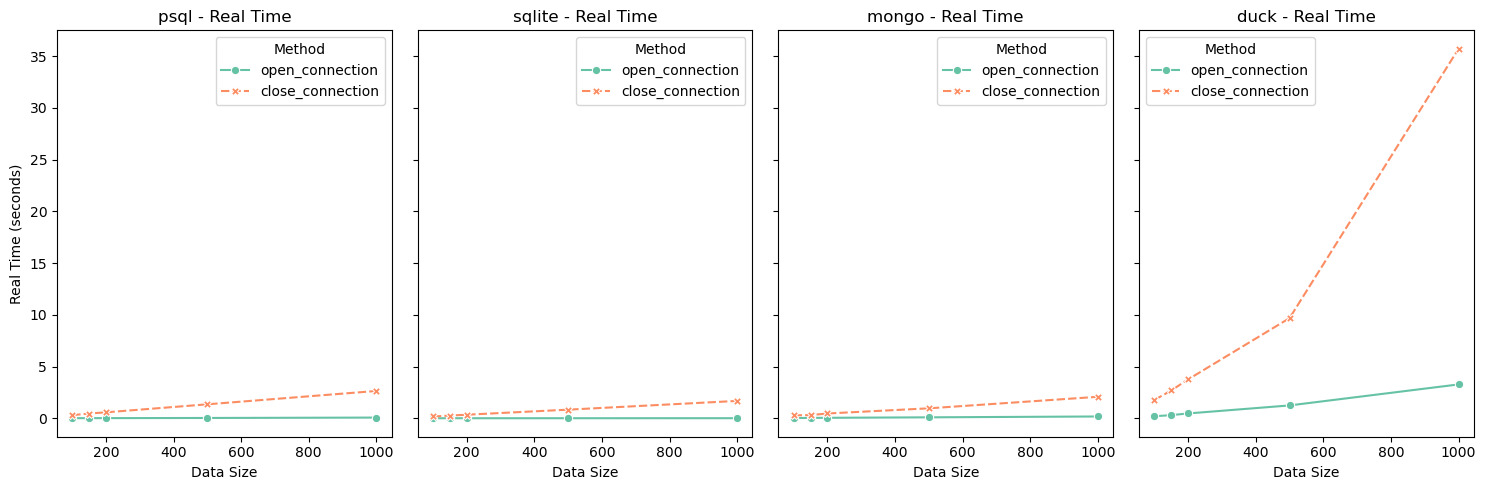
\includegraphics[width=0.8\textwidth]{img/page14_img1.png}
\caption{Comparative subplots of update operations, opening and closing connection, in different DBMSs}
\end{figure}

Updates of different database records are done with the same methods as read operations: \texttt{one} and \texttt{at\_once}. As we previously recounted, \texttt{one} is much slower than \texttt{at\_once}.

In theory, we studied that MongoDB is a document-oriented database, therefore, update performance depends on the document structure. Updates are at the document level, meaning the entire document must be rewritten to disk when modified. The UPDATE operation is therefore relatively fast compared to relational databases (SQLite and PostgreSQL) if only one document is modified; however, if the data to modify is referentially across several documents and a \ is required, it can be very slow, as we already verified in read operations.

In SQLite, we discovered that updates lock the entire database (we had to solve errors of this type), thus we believe it can affect performance and be slower than PostgreSQL. The use of indexes can improve performance as it makes it easier to find the record you wish to update.

We verified that in PostgreSQL, UPDATE operations perform well. We believe it might be due to its built-in transaction handling capabilities. The use of indexes makes update processes more efficient.

As seen in theoretical classes, DuckDB is designed for OLAP transactions and not for OLTP transactions. Even so, it supports update operations, but its performance is not optimized for high-volume transactions, as in MongoDB or PostgreSQL. DuckDB is not an index-oriented database like PostgreSQL or MongoDB. Therefore, updates are not usually affected by indexes, as data access is managed more at the columnar block level.

In general, indexes help improve the speed of finding the record we are going to update. However, if the updated field is indexed, the index also needs to be modified. In the case of updating the city, indexes speed up the operation since the city field was not indexed, whereas if we modify the ID, it will be costlier because it will have to update the index.

\section{Automation Pipeline}
Once all tests have been performed and tried separately, it is time to automate the testing process to replicate it with different parameters and databases. To do this, we designed the \texttt{AutoTester} class, which implements a \texttt{run\_tests()} method that sequentially executes everything developed above. This class will take as parameters the data input path (CSV for zip codes and cars), the data output paths (test results will be displayed on screen, but will also be saved in CSV format along with generated time plots), as well as other general configuration parameters such as iterations per test, DBMSs to consider, data provider or caches (pointers to created objects, if not automatically created in the class), test data sizes (passed in a dictionary, justified here).

Once created, we simply initialize an instance of this, \texttt{AutoTester()}, which we can even initialize without parameters (all present default values), and then invoke the \texttt{run\_tests()} method and see how different outputs for the tests are obtained.

\section{Design Decisions and Code Architecture}
To design the entire project, a modular architecture was chosen, seeking as much independence between components as possible. This is fundamental because, for codes or systems with slightly larger size or complexity, it is very easy to end up intertwining numerous functions, making the code impossible to debug or maintain.

Therefore, the code was separated into the modules \texttt{util}, with general-purpose functions and constants like queries to execute, \texttt{data\_generation}, which contains the provider classes, \texttt{data\_schema}, with the definition of the data schema (tables, MongoDB does not need it since it has schema-on-read and not on-write like PSQL, SQLite3, and DuckDB do), \texttt{db\_operations}, containing functions to execute CRUD operations on the 4 studied DBMSs, \texttt{testing} and \texttt{testing\_pipeline}, implementing testing functions and sequential process definition, and \texttt{cache\_implementation}, which implements functions and classes related to Memcached and custom cache. Technically, there is a last module, \texttt{connection}, which simply contains connection parameters for each DB to make it easier to change when sharing the project code among different programmers.

The main flow of the program takes place in an IPython notebook, \texttt{main.ipynb}, where the developed functions are imported and code is kept as short and concise as possible to more clearly present test outputs and concluded results.

Regarding design decisions, it should be noted that in DuckDB we could have used either a connection to a db file or to the computer\'s own memory. We opted to handle files in the development of this project.

\begin{figure}[h]
\centering
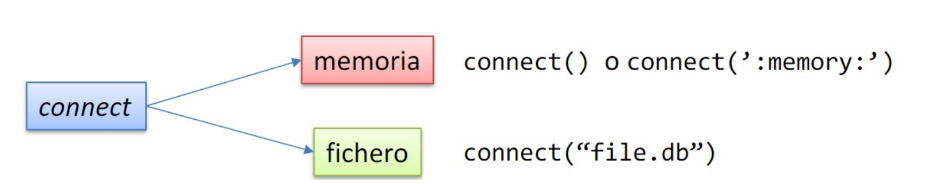
\includegraphics[width=0.8\textwidth]{img/page15_img1.png}
\caption{Diagram of possible two uses of DuckDB}
\end{figure}

Another design decision we made, logically, is that the methods of our Custom Cache have the same methods and parameters (i.e., an equivalent interface) as those provided by Memcached, since this allows reusing functions and procedures for both, reducing code redundancy and thus the possibility of errors.

Regarding the memory and time profiling functions provided in theory, they have been slightly modified, adding some optional parameter for the correct flow functioning (e.g., \texttt{both:bool = False}, since the insertion test cannot be done multiple times except with different data, due to primary key and uniqueness constraints, without deleting in between).

Lastly, and in the case of the testing pipeline, we decided that the sizes parameter should not be a simple \texttt{List[int]}, but represent a \texttt{Dict[str, List[int]]}, where keys (\texttt{'huge'}, \texttt{'big'}, \texttt{'small'}, \texttt{'ultra\_small'}) are associated with size lists. This was done to make testing practical, since, for example, data generation can easily be done with 1e6 data points (about 50 secs), while a query with JOINS on all records of a MongoDB collection would take several hours to execute with those amounts of observations.

\section{Conclusions}
In conclusion, the comparative analysis of database management systems SQLite, DuckDB, PostgreSQL, and MongoDB reveals that each possesses a unique data model and characteristics that make them suitable for different types of applications. For example, we observed in previous sections that MongoDB is very efficient when it comes to data insertion, while for complex queries like JOINS (ref section 5.3.1), it performs poorly compared to its relational counterparts.

When considering caching and indexing mechanisms, it is possible to further improve data management, but it does not always have to do so, as we verified in certain query tests (ref section 5.4). We conclude that choosing the right database system is, therefore, essential to optimize performance, as factors like data type, information volume, and access requirements can influence system efficiency.

\section{Bibliography}
\begin{enumerate}
\item PostgreSQL Global Development Group. PostgreSQL Documentation. \url{https://www.postgresql.org/docs/}
\item MongoDB, Inc. MongoDB Manual. \url{https://docs.mongodb.com/manual/}
\item SQLite Consortium. SQLite Documentation. \url{https://www.sqlite.org/docs.html}
\item DuckDB Community. DuckDB Documentation. \url{https://duckdb.org/docs/}
\item Memcached Team. Memcached: A distributed memory object caching system. \url{https://memcached.org/}
\item Sam Smith. Faker Documentation. \url{https://faker.readthedocs.io/en/master/}
\item The Pandas Development Team. Pandas Documentation. \url{https://pandas.pydata.org/docs/}
\item Travis E. Olliphant et al. NumPy Documentation. \url{https://numpy.org/doc/}
\item The Python Software Foundation. os — Miscellaneous operating system interfaces. \url{https://docs.python.org/3/library/os.html}
\item The Python Software Foundation. sys — System-specific parameters and functions. \url{https://docs.python.org/3/library/sys.html}
\item The Python Software Foundation. time — Time access and conversions. \url{https://docs.python.org/3/library/time.html}
\item Stack Overflow. Stack Overflow Community. \url{https://stackoverflow.com/}
\end{enumerate}

\end{document}
